

\section{Ejercicio 2}
	\begin{flushleft}
		\textit{Usando la información obtenida en el ejercicio anterior, obtener los parámetros del
espectrograma que permitan observar de la mejor manera posible las características tiempo-
frecuencia de este archivo de audio. Por medio de este espectrograma debe ser posible
identificar las siguientes notas del piano cuyas frecuencias aproximadas se representan en la Tabla \ref{tab:notas}.}
	\end{flushleft}

	\begin{table}[H]
		\centering
		\begin{tabular}{*{12}{c}}
			\toprule
			Do&Do\# &Re&Re\# &Mi&Fa&Fa\# &Sol&Sol\# &La&La\# &Si\\
			\midrule
			523&554&587&622&659&698&740&784&831&880&932&988\\
			1046&1108&1174&1244&1318&1386&1480&1568&1662&1760&1864&1976\\
			\bottomrule
		\end{tabular}
		\caption{Frecuencias que representan las notas musicales en su cuarta y quinta octava.}
		\label{tab:notas}
	\end{table}

	\subsection{Parámetros del espectrograma}
		De la Tabla \ref{tab:notas} se ve que el intervalo más corto de frecuencias es $554-523=31=\Delta f_{\min}$. Además por el Ejercicio \ref{sec:ej1}, se sabe que $\Delta t_{\min}=\SI{0.2}{\s}$. Por lo tanto:
		\begin{align*}
			F_S \cdot \SI{0.2}{\s} = \frac{F_S}{\SI{5}{\Hz}} > l_{ventana} &> \frac{F_S}{\SI{31}{\Hz}}\\
		\end{align*}

		Se propone utilizar $l_{ventana}=\frac{F_S}{\SI{10}{\Hz}}$ y resulta el gráfico de la Figura \ref{graf:spec_ej2}.
		Como criterio se propone un error relativo del 10\%. Si el error es menor, la representación se considerará correcta.

		\begin{figure}[h!]
			\centering
			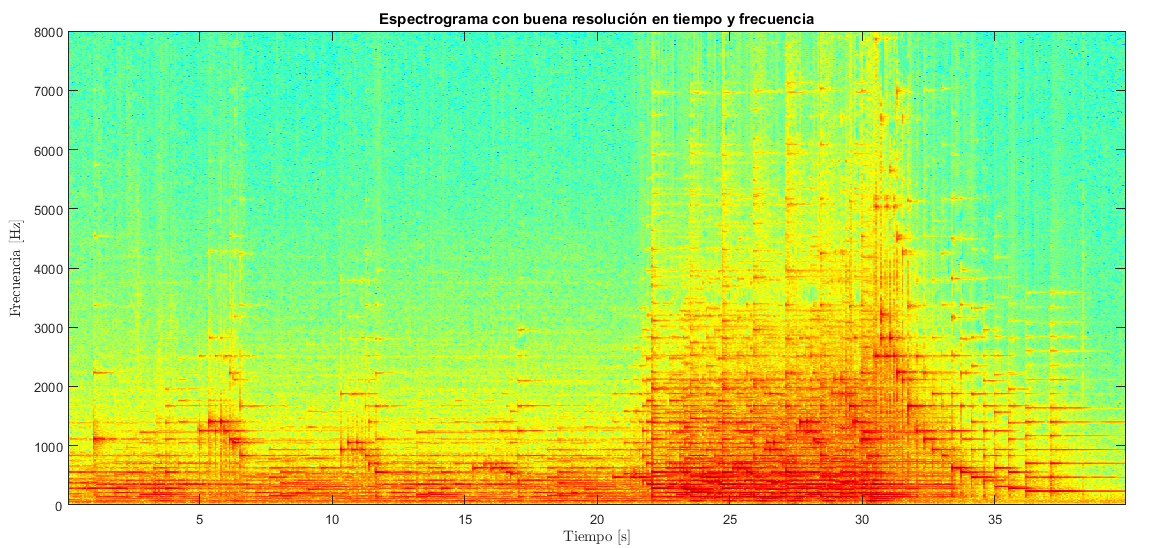
\includegraphics[scale=0.35]{2.png}
			\caption{Espectrograma de precisión.}
			\label{graf:spec_ej2}
		\end{figure}

	\subsection{Detección de las notas}
		Se buscaron las frecuencias que representan a las notas musicales en el espectograma y se obtuvieron sus valores más próximos expuestos en la Tabla \ref{tab:comparativa1} y sus respectivos errores en la Tabla \ref{tab:comparativa2}.

	\begin{table}[H]
		\centering
		\begin{tabular}{*{12}{c}}
			\toprule
			Do&Do\# &Re&Re\# &Mi&Fa&Fa\# &Sol&Sol\# &La&La\# &Si\\
			\midrule
			\num{523.44}&\num{554.69}&\num{585.94}&\num{625}&\num{656.25}&\num{695.31}&\num{742.19}&\num{781.25}&\num{828.13}&\num{882.81}&\num{929.69}&\num{992.19}\\
			\num{1046.9}&\num{1109.4}&\num{1171.9}&\num{1242.2}&\num{1320.3}&\num{1390.6}&\num{1484.4}&\num{1570.3}&\num{1664.1}&\num{1765.6}&\num{1867.2}&\num{1976.6}\\
			\bottomrule
		\end{tabular}
		\caption{Frecuencias del espectrograma más próximas a las de la tabla \ref{tab:notas}.}
		\label{tab:comparativa1}
	\end{table}

	\begin{table}[H]
		\centering
		\begin{tabular}{*{12}{c}}
			\toprule
			Do&Do\# &Re&Re\# &Mi&Fa&Fa\# &Sol&Sol\# &La&La\# &Si\\
			\midrule
			\num{0.4375}&\num{0.6875}&\num{1.0625}&\num{3}&\num{2.75}&\num{2.6875}&\num{2.1875}&\num{2.75}&\num{2.875}&\num{2.8125}&\num{2.3125}&\num{4.1875}\\
			\num{0.875}&\num{1.375}&\num{2.125}&\num{1.8125}&\num{2.3125}&\num{4.625}&\num{4.375}&\num{2.3125}&\num{2.0625}&\num{5.625}&\num{3.1875}&\num{0.5625}\\
			\bottomrule
		\end{tabular}
		\caption{Diferencia entre las frecuencias del espectrograma que representan a las notas y las reales.}
		\label{tab:comparativa2}
	\end{table}

	A partir de estas tablas se ve que la máxima diferencia es de \num{5.625} (5\textsuperscript{ta} octava del La) y el error relativo máximo es de 0,5\% (4\textsuperscript{ta} octava de Re). Al estar dentro del criterio propuesto, el espectograma permite identificar las notas requeridas.

